% -*- coding: utf-8 -*-

\begin{chapter}{Взаимодействие верхних слоев океана с ветром}\label{chap:9}
% \chapter{Response of the Upper Ocean to Winds}

Если вы когда-либо путешествовали по Соединенным Штатам, то могли
заметить, что климат восточного и западного побережий сильно отличается.
В чем же причина? Почему климат Чарльстона (Южная Каролина)
так мало похож на климат Сан-Диего (Калифорния), хотя оба они находятся
приблизительно на \latlon{32}{N} и на побережье или недалеко от океана? 
В Чарльстоне выпадает примерно $125$--$150\cm$ осадков ежегодно, 
а в Сан-Диего~--- $25$--$50\cm$, в Чарльстоне летом жарко, а в Сан-Диего, 
наоборот, прохладно. Или почему климат Сан-Франциско так отличен от климата
Норфолка (Вирджиния)?
%
% If you have had a chance to travel around the United States, you may
% have noticed that the climate of the east coast differs considerably
% from that on the west coast. Why? Why is the climate of Charleston,
% South Carolina so different from that of San Diego, although both are
% near 32\degrees N, and both are on or near the ocean? Charleston has
% 125--150 cm of rain a year, San Diego has 25--50 cm, Charleston has
% hot summers, San Diego has cool summers. Or why is the climate of San
% Francisco so different from that of Norfolk, Virginia?

Если повнимательнее рассмотреть характеристики атмосферы вдоль двух
берегов около \latlon{32}{N}, то становятся видны различия, которые могут
объяснить климат. Например, когда ветры с моря дуют прямо на Сан-Диего, 
они формируют пограничный слой толщиной несколько сотен метров, состоящий 
из прохладного влажного морского воздуха, над которым воздух намного суше и
теплее. В то же время, на восточном побережье, когда ветер дует с
моря, образующися здесь пограничный слой теплого влажного морского 
воздуха будет существенно толще. Конвекция, которая является предпосылкой 
возникновения осадков, протекает гораздо активнее на восточном побережье, 
чем на западном. Но почему атмосферный пограничный слой над поверхностью воды 
на восточном и западном побережьях столь различен? Ответ может быть найден 
в ходе изучения взаимодействия океана с локальными ветрами, которому посвящена
эта глава.
%
% If we look closely at the characteristics of the atmosphere along the
% two coasts near 32\degrees N, we find more differences that may
% explain the climate. For example, when the wind blows onshore toward
% San Diego, it brings a cool, moist, marine, boundary layer a few
% hundred meters thick capped by much warmer, dry air. On the east
% coast, when the wind blows onshore, it brings a warm, moist, marine,
% boundary layer that is much thicker. Convection, which produces rain,
% is much easier on the east coast than on the west coast. Why then is
% the atmospheric boundary layer over the water so different on the two
% coasts? The answer can be found in part by studying the ocean's
% response to local winds, the subject of this chapter.

\begin{section}{Инерционное движение}
% \section{Inertial Motion}
Прежде, чем начать изучение приповерхностных океанских течений, 
обсудим простейшее решение уравнений движения, описывающих
реакцию океана на импульс, приводящий воду в движение. 
Например, источником такого импульса может быть сильный ветер, дующий в 
течение нескольких часов. Он приводит воду в движение, а затем она движется 
под воздействием силы Кориолиса, без приложения к ней каких-либо других сил. 
%
% \index{inertial!motion}To begin our study of currents near the sea
% surface, let's consider first a very simple solution to the equations
% of motion, the response of the ocean to an impulse that sets the water
% in motion.  For example, the impulse can be a strong wind blowing for
% a few hours. The water then moves only under the influence of Coriolis
% force. No other force acts on the water.

Такое движение называется инерционным. Масса воды продолжает двигаться 
благодаря присущей ей инерции. Если бы эта жидкость находилась в космическом
пространстве, не взаимодействуя с другими телами, то она двигалась бы 
равномерно и прямолинейно согласно второму закону Ньютона. Если же требуется
учесть тот факт, что жидкость движется по поверхности вращающейся Земли, 
картина получается совсем иной.
%
% Such motion is said to be inertial. The mass of water continues to
% move due to its inertia. If the water were in space, it would move in
% a straight line according to Newton's second law. But on a rotating
% earth, the motion is much different.

Согласно~(\ref{eq:7.12}), уравнения движения частицы жидкости в океане 
при отсутствии трения имеют вид:
\begin{subequations}\label{eq:9.1}
\begin{align}
 \frac{du}{dt}&=-\frac{1}{\rho}\,\frac{\partial{p}}{\partial{x}} + 2\Omega v\,\sin\varphi, \\
 \frac{dv}{dt}&=-\frac{1}{\rho}\,\frac{\partial{p}}{\partial{y}} - 2\Omega u\,\sin\varphi, \\
 \frac{dw}{dt}&=-\frac{1}{\rho}\,\frac{\partial{p}}{\partial{z}} + 2\Omega u\,\cos\varphi - g,
\end{align}
\end{subequations}
где $p$~--- давление, 
$\Omega = 2\,\pi/\text{(звёздные сутки)} = 7.292\times 10^{-5}\radps$~--- 
скорость вращения Земли вокруг своей оси относительно неподвижной системы
координат и $\varphi$~--- широта.
%
% From (7.12) the equations of motion for a parcel of water moving in
% the ocean without friction are:
% \begin{subequations}
% \begin{align}
% \frac{du}{dt}&=-\frac{1}{\rho}\,\frac{\partial{p}}{\partial{x}} + 2\Omega v\,\sin\varphi \\
% \frac{dv}{dt}&=-\frac{1}{\rho}\,\frac{\partial{p}}{\partial{y}} - 2\Omega u\,\sin\varphi \\
% \frac{dw}{dt}&=-\frac{1}{\rho}\,\frac{\partial{p}}{\partial{z}} + 2\Omega u\,\cos\varphi - g
% \end{align}
% \end{subequations}
% where $p$ is pressure, $\Omega = 2\,\pi$/(sidereal day) $= 7.292
% \times 10^{-5}$ rad/s is the rotation of the earth in fixed
% coordinates, and $\varphi$ is latitude.

Попробуем найти простые решения этих уравнений. Чтобы это
сделать, требуется упростить уравнения количества движения. Прежде всего, 
отметим, что в жидкости, на которую воздействует только сила Кориолиса, 
проекция градиента давления на горизонтальную плоскость должна равняться нулю:
\begin{displaymath}
 \frac{\partial{p}}{\partial{x}} = \frac{\partial{p}}{\partial{y}} = 0.
\end{displaymath}
Далее, мы можем предположить, что течение плоское, в силу чего 
система~(\ref{eq:9.1}) принимает вид:
\begin{subequations}\label{eq:9.2}
 \begin{align}
  \frac{du}{dt}&= 2\Omega \,v \sin\varphi =  fv, \\
  \frac{dv}{dt}&=-2\Omega \,u \sin\varphi = -fu,
 \end{align}
\end{subequations}
где
\begin{equation}
 \boxed{f = 2\,\Omega\,\sin\varphi }
\end{equation}
называется \emph{параметром Кориолиса}\index{Кориолиса параметр|textbf},
а $\Omega = 7.292 \times 10^{-5}\radps$~---
%% в оригинале другая единица измерения, с^{-1}, но и так тоже вроде правильно,
%% т.к. радиан считается безразмерной величиной
скорость вращения Земли.
%
% Let's now look for simple solutions to these equations. To do this we
% must simplify the momentum equations. First, if only the Coriolis
% force acts on the water, there must be no horizontal pressure
% gradient:
% \begin{displaymath}
% \frac{\partial{p}}{\partial{x}} = \frac{\partial{p}}{\partial{y}} = 0
% \end{displaymath}
% Furthermore, we can assume that the flow is horizontal, and (9.1)
% becomes:
% \begin{subequations}
% \begin{align}
% \frac{du}{dt}&=2\Omega \,v \sin\varphi =fv \\
% \frac{dv}{dt}&=-2\Omega \,u \sin\varphi = -fu
% \end{align}
% \end{subequations}
% where:
% \begin{equation}
% \boxed{f = 2\,\Omega\,\sin\varphi }
% \end{equation}
% is the \textit{Coriolis Parameter}\index{Coriolis parameter|textbf}
% and $\Omega = 7.292 \times 10^{-5}$/s is the rotation rate of earth.

Система линейных дифференциальных уравнений первого порядка~(\ref{eq:9.2})
может быть решена стандартными методами. Найдем решение второго уравнения
относительно~$u$ и подставим его в первое, откуда мы получим
\begin{displaymath}
 \frac{du}{dt}=-\frac{1}{f}\,\frac{d^2v}{dt^2}=fv.
\end{displaymath}
Приведя уравнение к стандартному виду, получим уравнение гармонического
осциллятора:
\begin{equation}
 \frac{d^2v}{dt^2} + f^2v = 0,
\end{equation}
решение которого имеет вид~(\ref{eq:9.5}). 
Такое течение называется 
\emph{инерционным течением}\index{инерционное!течение|textbf} 
или \emph{инерционным колебанием}\index{инерционное!колебание|textbf}:
\begin{equation}\label{eq:9.5}
\boxed{\begin{aligned}
 u    &= V\, \sin ft, \\
 v    &= V\, \cos ft, \\
 V^2  &= u^2+v^2. \end{aligned}}
\end{equation}
Отметим, что уравнения~(\ref{eq:9.5}) задают в параметрической форме
окружность диаметром~$D_i = 2V/f$ и 
периодом~$T_i = (2\pi)/f = T_{sd}/(2\sin\varphi)$, 
где $T_{sd}$~--- длительность звездных суток.
%% что за "период" окружности?
%
% Equations (9.2) are two coupled, first-order, linear, differential
% equations which can be solved with standard techniques. If we solve
% the second equation for $u$, and insert it into the first equation we
% obtain:
% \begin{displaymath}
% \frac{du}{dt}=-\frac{1}{f}\,\frac{d^2v}{dt^2}=fv
% \end{displaymath}
% Rearranging the equation puts it into a standard form we should
% recognize, the equation for the harmonic oscillator:
% \begin{equation}
% \frac{d^2v}{dt^2} + f^2v = 0
% \end{equation}
% which has the solution (9.5). This current is called an
% \textit{inertial current}\index{inertial!current|textbf} or
% \textit{inertial oscillation}\index{inertial!oscillation|textbf}:
% \begin{equation}
% \fbox{$ \D \begin{aligned}%{cc}
% u &= V\, \sin ft \\
% v &= V\, \cos ft \\
% V^2  &= u^2+v^2 \end{aligned}$}
% \end{equation}
% Note that (9.5) are the parametric equations for a circle with
% diameter $D_i = 2V/f$ and period $T_i = (2\pi)/f=
% T_{sd}/(2\sin\varphi)$ where $T_{sd}$ is a sidereal day.

\begin{figure}[t]
\makebox[120mm] [c]{\includegraphics{pics/inertialcur}}
\caption{Инерционные течения в северной части Тихого океана 
(октябрь 1987~г., дни года 275--300), измеренные дрейфующим буем с плавучим
якорем типа <<дырявый носок>>, погруженным на глубину~$15\m$. Место буя 
определялось 10--12 раз в день при помощи системы Argos\index{Argos (система)}, 
установленной на метеорологических полярно-орбитальных спутниках NOAA. По этим
данным производилась интерполяция с интервалом~$3\hrs$. Сильнейшие течения,
зарегистрированные на 277-й день, возникли в результате шторма. Отметим, что
изображены не отдельные вихри. Вся поверхность вращается, и буй, выпущенный
в любой точке данного региона, был бы вовлечен в аналогичное вращательное 
движение. van Meurs (1998)}
\label{fig:inertialcur}
\end{figure}
%
% \begin{figure}[t]
% \makebox[120mm] [c]{\includegraphics{inertialcur}}
% \footnotesize
% Figure 9.1 Inertial currents \rule{0mm}{3ex}in the North Pacific in
% October 1987 (days 275--300) measured by holey-sock drifting buoys
% drogued at a depth of 15 meters. Positions were observed 10--12 times
% per day by the Argos system\index{Argos system} on \textsc{noaa}
% polar-orbiting weather satellites and interpolated to positions every
% three hours. The largest currents were generated by a storm on day
% 277. Note these are not individual eddies. The entire surface is
% rotating. A drogue placed anywhere in the region would have the same
% circular motion. After van Meurs (1998).
% \label{fig:inertialcur}
% \vspace{-3ex}
% \end{figure}

Величина~$T_i$ называется 
\emph{инерционным периодом}\index{инерционный!период|textbf}.
Она равна половине маятниковых суток, то есть времени, требуемого для
для полного оборота частицы по кругу инерции (табл.~\ref{tbl:9.1}). 
Направление вращения при этом 
\emph{антициклоническое}\index{антициклонический|textbf}: 
по часовой стрелке в северном полушарии и против часовой~--- в южном. 
Инерционное течение~--- это
свободное движение масс воды на вращающейся плоскости.
%
% $T_i$ is the \textit{inertial
% period}\index{inertial!period|textbf}. It is one half the time
% required for the rotation of a local plane on earth's surface (Table
% 9.1). The rotation is
% \textit{anti-cyclonic}\index{anti-cyclonic|textbf}: clockwise in the
% northern hemisphere, counterclockwise in the southern. Inertial
% currents are the free motion of parcels of water on a rotating plane.

\begin{table}[h]
\caption{Инерционные колебания}\label{tbl:9.1}
\begin{center}
\begin{tabular}{ccc}
\hline
Широта $(\varphi)$ & $T_i$ (ч) & $D$ (км) \\
                 & \multicolumn{2}{c}{для~$V = 20\cmps$} \\
\hline
$\degrees{90}$ & $11.97$ & $2.7$   \\
$\degrees{35}$ & $20.87$ & $4.8$   \\
$\degrees{10}$ & $68.93$ & $15.8$  \\
\hline
\end{tabular}
\end{center}
\end{table}
%
% \begin{table}[h!]\centering \small
% \vspace{-1ex}
% \begin{tabular*}{50mm}{@{}ccc@{}}
% \multicolumn{3}{@{}l@{}} {\bfseries Table 9.1 Inertial Oscillations} \\
% \hline
% Latitude $(\varphi)$ & $T_i$ (hr) & D\rule{0ex}{2.5ex} (km) \\
%                       & \multicolumn{2}{c}{for V = 20 cm/s} \\
% \hline
% 90\degrees & 11.97\rule{0ex}{2.5ex} & 2.7 \\
% 35\degrees & 20.87 & 4.8  \\
% 10\degrees & 68.93 & 15.8  \\ [0.5ex]
% \hline
% \end{tabular*} \\[0.5ex]
% \vspace{-3ex}
% \end{table}

Инерционные течения\index{инерционное!течение}~--- наиболее распространенные 
течения в океане (рис.~\ref{fig:inertialcur}). Вебстер Webster (1968) 
проанализировал множество опубликованных работ по данной тематике
и обнаружил, что такие течения наблюдались на всех глубинах и под всеми
широтами, но они непостоянны и затухают в течение нескольких
дней. Колебания на различных глубинах или в различных близко расположенных
точках, как правило, некогерентны.
%
% Inertial currents are the most common currents in the ocean (figure
% 9.1). Webster (1968) reviewed many published reports of inertial
% currents\index{inertial!current} and found that currents have been
% observed at all depths in the ocean and at all latitudes. The motions
% are transient and decay in a few days. Oscillations at different
% depths or at different nearby sites are usually incoherent.

Причиной возникновения инерционных течений является резкая смена ветра
у поверхности моря; при этом быстрая перемена сильных ветров порождает
наибольшие колебания. Несмотря на то, что при выводе уравнений колебаний мы
предполагали, что трение отсутствует, полностью его игнорировать невозможно.
Со временем колебания вырождаются в другие поверхностные течения. 
Подробнее эти явления рассматриваются в работе Apel, 1987: \S6.3.
%
% Inertial currents are caused by rapid changes of wind at the sea
% surface, with rapid changes of strong winds producing the largest
% oscillations. Although we have derived the equations for the
% oscillation assuming frictionless flow, friction cannot be completely
% neglected. With time, the oscillations decay into other surface
% currents. (See, for example, Apel, 1987: \S6.3 for more information.)
\end{section}

\begin{section}{Приповерхностный слой Экмана}
% \section{Ekman Layer at the Sea Surface}
Устойчивые ветры, \index{Экмана слой|(}дующие над поверхностью 
океана, \index{Экмана слой!поверхность моря|(} порождают тонкий горизонтальный
пограничный слой, который называется \textit{слоем Экмана}. 
\index{Экмана слой!определение|textbf} Под <<тонким>> в данном контексте
подразумевается слой с толщиной, не превышающей нескольких сотен метров, 
что по сравнению с глубиной океана достаточно мало. Аналогичный пограничный
слой существует и возле океанского дна; он получил название 
\emph{придонного слоя Экмана}\index{Экмана слой!придонный|textbf}.
Наконец, еще один слой Экмана располагается в нижних слоях атмосферы 
непосредственно над поверхностью моря: планетарный пограничный слой
%% ??? Х-М: слой Экмана расположен выше, с поверхностью моря контактирует
%% приземный/приводный слой
или слой трения, описанный в разд.~\ref{sec:BoundaryLayer}. Слой Экмана 
был назван в честь Вальфрида Экмана, который исследовал его 
динамику в своей докторской диссертации.
%
% Steady winds \index{Ekman layer|(}blowing on \index{Ekman layer!sea
% surface|(}(the sea surface produce a thin, horizontal boundary layer,
% the \textit{Ekman layer}. \index{Ekman layer!defined|textbf} By thin,
% I mean a layer that is at most a few-hundred meters thick, which is
% thin compared with the depth of the water in the deep ocean. A similar
% boundary layer exists at the bottom of the ocean, the \textit{bottom
% Ekman layer}\index{Ekman layer!bottom|textbf}, and at the bottom of
% the atmosphere just above the sea surface, the planetary boundary
% layer or frictional layer described in \S 4.3. The Ekman layer is
% named after Professor Walfrid Ekman, who worked out its dynamics for
% his doctoral thesis.

Работа Экмана была первой в ряду исследований, проведенных в первой половине
XX~столетия, которые заложили основы понимания роли ветров в циркуляции
океана (табл.~\ref{tbl:9.2}). В этой главе мы рассмотрим труды Ф.~Нансена
и В.~Экмана, а все прочие~--- в гл.\ref{chap:11} и~\ref{chap:13}.
%
% Ekman's work was the first of a remarkable series of studies conducted
% during the first half of the twentieth century that led to an
% understanding of how winds drive the ocean's circulation (Table
% 9.1). In this chapter we consider Nansen and Ekman's work. The rest of
% the story is given in chapters 11 and 13.

\begin{table}[t!]
\caption{Вклад в теорию ветровой циркуляции}\label{tbl:9.2}
\begin{footnotesize}
\begin{tabular}{p{0.255\textwidth}p{0.05\textwidth}p{0.6\textwidth}}
\hline
Фритьоф Нансен     & (1898) 
  & Качественная теория переноса воды течениями под углом к направлению ветра. \\
Вагн Вальфрид Экман & (1902)    
  & Количественная теория ветрового переноса\index{перенос!ветровой} 
    на морской поверхности. \\
Харальд Свердруп     & (1947)
  & Теория ветровой циркуляции в восточной части Тихого океана. \\
Генри Стоммел   & (1948)     
  & Теория западной интенсификации ветровой циркуляции
    (западные пограничные течения). \\
Уолтер Манк  & (1950)
  & Количественная теория основных свойств ветровой циркуляции. \\
Кирк Брайен  & (1963)
  & Численные модели океанской циркуляции. \\
Берт Семтнер, \goodbreak Роберт Червин & (1988) 
  & Глобальная вихреразрешающая реалистическая модель океанской циркуляции. \\
\hline
\end{tabular}
\end{footnotesize}
\end{table}
%
% \begin{table}[t!]\small
% \begin{tabular*}{120mm}{@{}lcl@{}}
% \multicolumn{3}{@{}l@{}}{\bfseries Table 9.2 Contributions to the Theory of the
% \rule[-1ex]{0mm}{1ex}Wind-Driven Circulation}  \\
% \hline
% Fridtjof Nansen     & (1898)    & Qualitative \rule{0ex}{2.5ex}theory, currents transport water at an \\
% &&\hspace{1em}angle to the wind. \\
% Vagn Walfrid Ekman  & (1902)    & Quantitative theory for wind-driven
% transport\index{transport!wind-driven} at \\ &&\hspace{1em}the sea surface. \\
% Harald Sverdrup     & (1947)    & Theory for wind-driven circulation in the eastern \\
% &&\hspace{1em}Pacific. \\
% Henry Stommel   & (1948)     & Theory for westward intensification of wind-driven \\
% &&\hspace{1em}circulation (western boundary currents). \\
% Walter Munk  & (1950)   & Quantitative theory for main features of the wind- \\
% &&\hspace{1em}driven circulation. \\
% Kirk Bryan  & (1963)    & Numerical models of the oceanic circulation. \\
% Bert Semtner & (1988) & Global, eddy-resolving, realistic model of the \\
%  \ \ and Robert Chervin &&\hspace{1em}ocean's circulation. \\
% \hline
% \end{tabular*} \\[0.5ex]
% \vspace{-3ex}
% \end{table}

\begin{paragraph}{Качественная теория Нансена.}
% \paragraph{Nansen's Qualitative Arguments}
Фритьоф Нансен отметил, что дрейф льдов в Арктике происходит под 
углом~$\degrees{20}$--$\degrees{40}$ вправо от направления ветра,
то есть, траектория движения айсберга отклоняется вправо, если смотреть
в направлении ветра (рис.~\ref{fig:forcesketch}). В дальнейшем он определил,
какое равновесие сил должно существовать при движении айсбергов
по поверхности вращающейся Земли под воздействием ветра.
%
% Fridtjof Nansen noticed that wind tended to blow ice at an angle of
% 20\degrees--40\degrees\ to the right of the wind in the Arctic, by
% which he meant that the track of the iceberg was to the right of the
% wind looking downwind (See figure 9.2). He later worked out the
% balance of forces that must exist when wind tried to push icebergs
% downwind on a rotating earth.

Согласно теории Нансена, в данном процессе существенно влияние трех сил:
% Nansen argued that three forces must be important:
\begin{enumparen}
\item ветровое напряжение~$\mbfW$;
%
% \vitem Wind Stress, \textbf{W};

\item 
сила трения~$\mbfF$ (при отсутствии трения айсберг перемещался бы со скоростью
ветра);
%
% \vitem Friction \textbf{F} (otherwise the iceberg would move as fast
% as the wind);

\item 
сила Кориолиса\index{Кориолиса сила}~$\mbfC$.
%
% \vitem Coriolis Force\index{Coriolis force}, \textbf{C}.
\end{enumparen}
Далее, Нансен утверждал, что этим силам должны быть присущи следующие 
свойства:
%
% Nansen argued further that the forces must have the following
% attributes:
\begin{enumerate}
\item 
Сила трения направлена противоположно вектору скорости.
%
% \vitem Drag must be opposite the direction of the ice's velocity;

\item 
Сила Кориолиса действует перпендикулярно вектору скорости.
%
% \vitem Coriolis force must be perpendicular to the velocity;

\item 
В случае установившегося течения силы уравновешиваются:  
\begin{displaymath}
 \mbfW + \mbfF + \mbfC = 0.
\end{displaymath}
%
% \vitem The forces must balance for steady flow.
\end{enumerate}
% \begin{center}
% \textbf{W} + \textbf{F} + \textbf{C} = 0
% \end{center}
\end{paragraph}

\begin{paragraph}{Результаты Экмана.}
% \paragraph{Ekman's Solution}
\index{Экмана слой!теория}Нансен предложил Вильгельму Бьеркнесу поручить
одному из своих студентов провести теоретическое исследование влияния вращения
Земли на ветровые течения. Для этой работы был выбран Вальфрид Экман, который
представил результаты в рамках своей диссертации, которую он защитил 
в Уппсале (Kullenberg, 1954). Впоследствии Экман развил свою теорию, дополнив 
%% "защитил"? или просто "писал"?
ее учетом влияния континентов и различий в плотности воды (Ekman, 1905). 
Дальнейшее изложение будет следовать рассуждениям Экмана, приведенным 
в его работе.
%
% Nansen \index{Ekman layer!theory of}asked Vilhelm Bjerknes to let one
% of Bjerknes' students make a theoretical study of the influence of
% earth's rotation on wind-driven currents. Walfrid Ekman was chosen,
% and he presented the results in his thesis at Uppsala (Kullenberg,
% 1954). Ekman later expanded the study to include the influence of
% continents and differences of density of water (Ekman, 1905). The
% following follows Ekman's line of reasoning in that paper.

\begin{figure}[t!]
\centering
\makebox[120mm] [c]{\includegraphics{pics/forcesketch}}
\caption{Равновесие сил, действующих на айсберг, движущийся под действием
ветра по поверхности вращающейся Земли.}
\label{fig:forcesketch}
\vspace{-3ex}
\end{figure}
%
% \begin{figure}[t!]
% \centering
% \makebox[120mm] [c]{\includegraphics{forcesketch}}
% \footnotesize
% Figure 9.2 The balance of forces \rule{0mm}{3ex}acting on an iceberg
% in a wind on a rotating earth.
%
% \label{fig:forcesketch}
% \vspace{-3ex}
% \end{figure}

Экман предположил\index{Экмана слой!Экмана предположения}, что течение на
поверхности вращающейся Земли будет установившимся, однородным и 
горизонтальным, а сила трения~--- существенной. Как следствие,
производные по горизонтальным и временной компонентам обращаются в нуль:
\begin{equation}
 \frac{\partial}{\partial{t}}=\frac{\partial}{\partial{x}}=\frac{\partial}{\partial{y}}=0.
\end{equation}
С учетом данных предположений, силы трения и Кориолиса 
на поверхности вращающейся Земли будут находиться 
в равновесии~(\ref{eq:8.15}). Еще одно предположение Экмана состояло в том, 
что вертикальная вихревая вязкость постоянна и имеет вид~(\ref{eq:8.13}):
\begin{equation}\label{eq:9.7}
 T_{xz} \,=\,\rho\, A_z \,\frac{\partial{u}}{\partial{z}}\: , \qquad 
 T_{yz} \,=\,\rho\, A_z \,\frac{\partial{v}}{\partial{z}},
\end{equation}
где~$T_{xz}$ и~$T_{yz}$~--- компоненты ветрового напряжения
\index{ветровое напряжение!компоненты} в направлениях~$x$ и~$y$,
а $\rho$~--- плотность морской воды.
%
% Ekman assumed\index{Ekman layer!Ekman's assumptions} a steady,
% homogeneous, horizontal flow with friction on a rotating earth. Thus
% horizontal and temporal derivatives are zero:
% \begin{equation}
% \frac{\partial}{\partial{t}}=\frac{\partial}{\partial{x}}=\frac{\partial}{\partial{y}}=0
% \end{equation}
% For flow on a rotating earth, this leaves a balance between frictional
% and Coriolis forces (8.15).  Ekman further assumed a constant vertical
% eddy viscosity of the form (8:13):
% \begin{equation}
% T_{xz} \,=\,\rho\, A_z \,\frac{\partial{u}}{\partial{z}}\: , \qquad T_{yz}\,=\,\rho\, A_z \,\frac{\partial{v}}{\partial{z}}
% \end{equation}
% where $T_{xz}$, $T_{yz}$ are the components of the wind
% stress\index{wind stress!components} in the $x$, $y$ directions, and
% $\rho$ is the density of sea water.

Подставив~(\ref{eq:9.7}) в~(\ref{eq:8.15}), получаем уравнения количества
движения по координатам~$x$ и~$y$:
\begin{subequations}\label{eq:9.8}
\begin{align}
  fv +  A_z \, \frac{\partial{^2 u}}{\partial{z^2}} &= 0, \\
  -fu + A_z \, \frac{\partial{^2 v}}{\partial{z^2}} &= 0,
\end{align}
\end{subequations}
где~$f$~--- параметр Кориолиса\index{Кориолиса параметр}.
%
% Using (9.7) in (8.15), the $x$ and $y$ momentum equations are:
% \begin{subequations}
% \begin{align}
% fv +  A_z \, \frac{\partial{^2 u}}{\partial{z^2}} &= 0  \\
% -fu + A_z \, \frac{\partial{^2 v}}{\partial{z^2}} &= 0
% \end{align}
% \end{subequations}
% where $f$ is the Coriolis parameter\index{Coriolis parameter}.

Легко убедиться в том, что уравнения~(\ref{eq:9.8}) имеют решения:
%% в оригинале (9.9)
\begin{subequations}
\begin{align}
 u &=  V_0\,\exp(az)\,\cos(\pi/4 + az),  \\
 v &=  V_0\,\exp(az)\,\sin(\pi/4 + az),
\end{align}
\end{subequations}
при условии, что ветер дует в северном направлении~$(T = T_{yz})$. 
Входящие в это решение константы равны, соответственно,
\begin{equation}\label{eq:9.10}
 V_0 = \frac{T}{\sqrt{\rho^2_w\,f\,A_z}} \qquad \text{и} \qquad
 a=\sqrt{\frac{f}{2A_z}},
\end{equation}
причем $V_0$~представляет собой абсолютную величину скорости течения 
на морской поверхности.
%
% It is easy to verify that the equations (9.9) have solutions:
% \begin{subequations}
% \begin{align}
% u &=  V_0\,\exp(az)\,\cos(\pi/4 + az)  \\
% v &=  V_0\,\exp(az)\,\sin(\pi/4 + az)
% \end{align}
% \end{subequations}
% when the wind is blowing to the north $(T = T_{yz})$. The constants
% are
% \begin{equation}
% V_0 = \frac{T}{\sqrt{\rho^2_w\,f\,A_z}} \qquad \text{and} \qquad
% a=\sqrt{\frac{f}{2A_z}}
% \end{equation}
% and $V_0$ is the velocity of the current at the sea surface.

Исследуем форму, которую имеют найденные решения. На морской 
поверхности $z = 0$, следовательно, $\exp(z=0) = 1$ и
\begin{subequations}
\begin{align}
u(0) &= V_0\, \cos(\pi/4),  \\
v(0) &= V_0\, \sin(\pi/4).
\end{align}
\end{subequations}
Таким образом, скорость течения равна~$V_0$, а его направление~--- 
к северо-востоку. В общем случае, в северном полушарии поверхностное течение 
направлено под углом~$\degrees{45}$ вправо от направления ветра, 
а в южном~--- влево. Под поверхностью скорость течения убывает с глубиной
по экспоненциальному закону (рис.~\ref{fig:ekmancurrent}):
\begin{equation}
 \left[u^2(z) + v^2(z) \right]^{1/2} =V_0\,\exp(az).
\end{equation}
%
% Now let's look at the form of the solutions. At the sea surface $z = 0$,
% $\exp(z=0) = 1$, and
% \begin{subequations}
% \begin{align}
% u(0) &= V_0\, \cos(\pi/4)  \\
% v(0) &= V_0\, \sin(\pi/4)
% \end{align}
% \end{subequations}
% The current has a speed of $V_0$ to the northeast. In general, the
% surface current is 45\degrees\ to the right of the wind when looking
% downwind in the northern hemisphere. The current is 45\degrees\ to the
% left of the wind in the southern hemisphere. Below the surface, the
% velocity decays exponentially with depth (figure 9.3):
% \begin{equation}
% \left[u^2(z) + v^2(z) \right]^{1/2} =V_0\,\exp(az)
% \end{equation}

\begin{figure}[h!]
\makebox[121mm] [c]{\includegraphics{pics/ekmancurrent}}
\caption{Экмановское течение, порождаемое ветром скоростью~$10\mps$ 
под~\latlon{35}{N}.}
\label{fig:ekmancurrent}
\end{figure}
%
% \begin{figure}[h!]
% \makebox[121mm] [c]{\includegraphics{ekmancurrent}}
% \centering
% \footnotesize
% Figure 9.3. Ekman current \rule{0mm}{4ex}generated by a 10 m/s wind at
% 35\degrees\ N.
%
% \label{fig:ekmancurrent}
% \end{figure}
\end{paragraph}

\begin{paragraph}{Величины констант Экмана.}
% \paragraph{Values for Ekman's Constants}
\index{Экмана слой!поверхностные константы}%
Дальнейшее изложение потребует знания любых двух из трех параметров:
скорости течения на поверхности~$V_0$, коэффициента вихревой вязкости~$A_z$
или ветрового напряжения\index{ветровое напряжение!и слой Экмана}~$T$.
%
% To proceed further, \index{Ekman layer!surface-layer constants}we need
% values for any two of the free parameters: the velocity at the
% surface, $V_0$; the coefficient of eddy viscosity, $A_z$; or the wind
% stress\index{wind stress!and Ekman layer} $T$.

Ветровое напряжение\index{ветровое напряжение!и слой Экмана} изучено хорошо,
поэтому Экман воспользовался приближенной формулой~(\ref{eq:4.2}):
\begin{equation}\label{eq:9.13}
 T_{yz} = T = \rho_{a}\, C_D \,U_{10}^2,
\end{equation}
где~$\rho_{a}$~--- плотность воздуха, $C_D$~--- коэффициент 
сопротивления\index{сопротивление!коэффициент}, а~$U_{10}$~--- скорость
ветра на высоте~$10\m$ над уровнем моря. Обратившись к литературе, Экман
обнаружил следующий способ вычисления~$V_0$ как функции скорости ветра:
\begin{equation}\label{eq:9.14}
 V_0 = \frac{0.0127}{\sqrt{\sin|\varphi|}}\, U_{10}, 
  \qquad \qquad |\varphi|\ge 10.
\end{equation}
%
% The wind stress\index{wind stress!and Ekman layer} is well known, and
% Ekman used the bulk formula (4.2):
% \begin{equation}
% T_{yz} = T = \rho_{air}\, C_D \,U_{10}^2
% \end{equation}
% where $\rho_{air}$ is the density of air, $C_D$ is the drag
% coefficient\index{drag!coefficient}, and $U_{10}$ is the wind speed at
% 10 m above the sea. Ekman turned to the literature to obtain values
% for $V_0$ as a function of wind speed. He found:
% \begin{equation}
% V_0 = \frac{0.0127}{\sqrt{\sin|\varphi|}}\, U_{10}, \qquad \qquad
% |\varphi|\ge 10
% \end{equation}

Используя эту формулу, он смог вычислить скорость как функцию глубины при
условии, что известны скорость ветра~$U_{10}$ и его направление.
%
% With this information, he could then calculate the velocity as a
% function of depth knowing the wind speed $U_{10}$ and wind direction.
\end{paragraph}

\begin{paragraph}{Глубина слоя Экмана.}
% \paragraph{Ekman Layer Depth}
\index{Экмана слой!глубина|textbf}Толщина слоя Экмана может быть произвольной,
поскольку скорость течений Экмана убывает с глубиной по экспоненте.
Экман предложил считать толщиной слоя Экмана глубину~$D_E$, на которой вектор
скорости течения направлен противоположно вектору скорости на поверхности,
что происходит на глубине~$D_E = \pi/a$. Таким образом,
\textit{глубина слоя Экмана}:
\begin{equation}\label{eq:9.15}
 \boxed{D_E = \sqrt{\frac{2\pi^2\,A_z}{f}}.}
\end{equation}
%
% \index{Ekman layer!depth|textbf}The thickness of the Ekman layer is
% arbitrary because the Ekman currents decrease exponentially with
% depth. Ekman proposed that the thickness be the depth $D_E$ at which
% the current velocity is opposite the velocity at the surface, which
% occurs at a depth $D_E = \pi/a$, and the \textit{Ekman layer depth}
% is:
% \begin{equation}
% \boxed{D_E = \sqrt{\frac{2\pi^2\,A_z}{f}}}
% \end{equation}

Подставив~(\ref{eq:9.13}) в~(\ref{eq:9.10}), разделив на~$U_{10}$, 
и воспользовавшись соотношениями~(\ref{eq:9.14}) и~(\ref{eq:9.15}), получим:
\begin{equation}\label{eq:9.16}
 D_E = \frac{7.6}{\sqrt{\sin|\varphi|}}\, U_{10}
\end{equation}
в единицах системы СИ. Скорость ветра, измеренная в м/с, дает глубину в метрах.
Коэффициент в~(\ref{eq:9.16}) вычислен, исходя из $\rho = 1027\kgpcm$, 
$\rho_{a} = 1.25\kgpcm$ и коэффициента 
сопротивления\index{сопротивление!коэффициент}, который был принят
Экманом равным $C_D = 2.6 \times 10^{-3}$.
%
% Using (9.13) in (9.10), dividing by $U_{10}$, and using (9.14) and
% (9.15) gives:
% \begin{equation}
% D_E = \frac{7.6}{\sqrt{\sin|\varphi|}}\, U_{10}
% \end{equation}
% in SI units. Wind in meters per second gives depth in meters. The
% constant in (9.16) is based on $\rho = 1027 $ kg/m$^3$, $\rho_{air} =
% 1.25 $ kg/m$^3$, and Ekman's value of $C_D = 2.6 \times 10^{-3}$ for
% the drag coefficient\index{drag!coefficient}.

Применив~(\ref{eq:9.16}) к типичным ветрам, получим, что толщина слоя Экмана
лежит в диапазоне~$45$--$300\m$ (табл.~\ref{tbl:9.3}), а поверхностная скорость 
составляет $2.5$--$1.1$\% скорости ветра в зависимости от 
широты\index{Экмана слой!морская поверхность|)}.
%
% Using (9.16) with typical winds, the depth of the Ekman layer varies
% from about 45 to 300 meters (Table 9.3), and the velocity of the
% surface current varies from 2.5\% to 1.1\% of the wind speed depending
% on latitude\index{Ekman layer!sea surface|)}.

\begin{table}[h!]
\caption{Типичные значения глубины Экмана}\label{tbl:9.3}
\begin{center}
\begin{tabular}{c|cc}
\hline
               &\multicolumn{2}{c}{Широта}      \\
$U_{10}\mps$  & $\degrees{15}$      & $\degrees{45}$ \\
\hline
5              & $75\m$  & $45\m$       \\
10             & $150\m$ & $90\m$       \\
20             & $300\m$ & $180\m$      \\
\hline
\end{tabular}
\end{center}
\end{table}
%
% \begin{table}[h!]\small \centering
% \vspace{-1ex}
% \begin{tabular*}{60mm}{@{}c|cc}
% \multicolumn{3}{@{}c@{}}{\bfseries Table 9.3 Typical Ekman Depths \rule[-1ex]{0mm}{1ex}}  \\
% \hline
%                &\multicolumn{2}{c}{Latitude}      \\
% U$_{10}$ [m/s]  & 15\degrees          & 45\degrees \\
% \hline
% 5              & \rule{0ex}{3ex}75  m & 45 m       \\
% 10             &                150 m & 90 m       \\
% 20             &                300 m & 180 m      \\
% \hline
% \end{tabular*} \\[0.5ex]
% \vspace{-3ex}
% \end{table}
\end{paragraph}

\begin{paragraph}{Число Экмана: силы Кориолиса и трения.}
% \paragraph{The Ekman Number: Coriolis and Frictional Forces}
Глубина слоя Экмана тесно связана с глубиной, на которой сила трения 
уравновешивается силой Кориолиса\index{Кориолиса сила} в уравнении количества
движения~(\ref{eq:9.8}). Сила Кориолиса равна~$f u$, а сила 
%% в оригинале 9.9
трения~--- $A_z \partial^2 U/\partial z^2$. Безразмерная величина, равная
отношению этих сил, называется 
\emph{числом Экмана}\index{Экмана число|textbf}~$E_z$:
\begin{displaymath}
 E_z= \frac{\text{сила трения}}{\text{сила Кориолиса}} 
    = \frac{A_z\frac{\partial^2u}{\partial{z^2}}}{fu} 
    = \frac{A_z\frac{u}{d^2}}{fu},
\end{displaymath}
\begin{equation}\label{eq:9.17}
 \boxed{E_z = \frac{A_z}{f\,d^2},}
\end{equation}
где мы воспользовались для вычисления приближенного значения типичными
величинами скорости~$u$ и глубины~$d$. Индекс~$z$ требуется потому, что океан
стратифицирован, и вертикальное перемешивание существенно меньше, 
чем горизонтальное. Отметим, что с ростом глубины трение ослабевает, так что
в итоге остается лишь воздействие силы Кориолиса.
%
% The depth of the Ekman layer is closely related to the depth at which
% frictional force is equal to the Coriolis force\index{Coriolis force}
% in the momentum equation (9.9). The Coriolis force is $f u$, and the
% frictional force is $A_z \partial^2 U/\partial z^2$. The ratio of the
% forces, which is non dimensional, is called the \textit{Ekman
% Number}\index{Ekman Number|textbf} $E_z$:
% \begin{displaymath}
% E_z=\frac{\text{Friction Force}}{\text{Coriolis Force}} = \frac{\D A_z\frac{\D\partial^2u}{\partial{z^2}}}{fu} = \frac{\D A_z\frac{\D
% u}{\D d^2}}{\D fu}
% \end{displaymath}
% \begin{equation}
% \boxed{E_z = \frac{A_z}{f\,d^2}}
% \end{equation}
% where we have approximated the terms using typical velocities $u$, and
% typical depths $d$. The subscript $z$ is needed because the ocean is
% stratified and mixing in the vertical is much less than mixing in the
% horizontal. Note that as depth increases, friction becomes small, and
% eventually, only the Coriolis force remains.

Решив~(\ref{eq:9.17}) относительно~$d$, получаем
\begin{equation}\label{eq:9.18}
 d = \sqrt{\frac{A_z}{fE_z}},
\end{equation}
что согласуется с зависимостью~(\ref{eq:9.15}), предложенной Экманом.
Чтобы величины~(\ref{eq:9.18}) и~(\ref{eq:9.15}) были равны, необходимо, чтобы 
на глубине Экмана $E_z = 1/(2\pi^2) \approx 0.05$. Следовательно, 
%% в оригинале вместо \approx стоит "=", но это же неверно...
Экман выбрал такую глубину, на которой силы трения гораздо слабее силы 
Кориолиса.
%
% Solving (9.17) for $d$ gives
% \begin{equation}
% d = \sqrt{\frac{A_z}{fE_z}}
% \end{equation}
% which agrees with the functional form (9.15) proposed by
% Ekman. Equating (9.18) and (9.15) requires $E_z = 1/(2\pi^2) = 0.05$
% at the Ekman depth. Thus Ekman chose a depth at which frictional
% forces are much smaller than the Coriolis force.
\end{paragraph}

\begin{paragraph}{Придонный слой Экмана.}
% \paragraph{Bottom Ekman Layer}
\index{Экмана слой!придонный}Слой Экмана на дне океана и в нижних слоях 
атмосферы отличаются от слоя возле поверхности океана. Для придонного слоя,
расположенного под жидкостью со скоростью течения~$U$ в направлении оси~$x$,
получаем:
\begin{subequations}
\begin{align}
 u&=U[1 - \exp(-az)\,\cos\,az],  \\
 v&=U\,\exp(-az)\,\sin\,az.
\end{align}
\end{subequations}
На границе скорость снижается до нуля ($u = v = 0$ при~$z = 0$). Направление
течения, близкого к границе, составляет угол в~$\degrees{45}$ влево от 
направления течения~$U$ за пределами пограничного слоя в северном полушарии,
а с изменением расстояния течение изменяет и свое 
направление (рис.~\ref{fig:bottomekman}). Направление поворота~--- 
антициклоническое, с ростом расстояния от нижней границы.
%
% \index{Ekman layer!bottom}The Ekman layer at the bottom of the ocean
% and the atmosphere differs from the layer at the ocean surface. The
% solution for a bottom layer below a fluid with velocity $U$ in the
% $x$-direction is:
% \begin{subequations}
% \begin{align}
% u&=U[1 - \exp(-az)\,\cos\,az]  \\
% v&=U\,\exp(-az)\,\sin\,az
% \end{align}
% \end{subequations}
% The velocity goes to zero at the boundary, $u = v = 0$ at $z = 0$. The
% direction of the flow close to the boundary is 45\degrees\ to the left
% of the flow $U$ outside the boundary layer in the northern hemisphere,
% and the direction of the flow rotates with distance above the boundary
% (figure 9.4). The direction of rotation is anti\-cyclonic with
% distance above the bottom.

\begin{figure}[b!]
\makebox[121mm][c]{\includegraphics{pics/bottomekman}}
\caption{Слой Экмана в нижнем слое атмосферы толщиной~$1\km$ (сплошная линия) 
и скорость ветра (штриховая линия), измеренные Добсоном Dobson (1914).
Числами задается высота над поверхностью в метрах. Слой Экмана вблизи дна 
океана имеет схожую форму. Согласно Houghton (1977: 107)}
\label{fig:bottomekman}
\end{figure}
%
% \begin{figure}[b!]
% \makebox[121mm] [c]{\includegraphics{bottomekman}}
% \footnotesize
% Figure 9.4 Ekman \rule{0mm}{3ex}layer in the lowest kilometer of the
% atmosphere (solid line), with wind velocity measured by Dobson (1914)
% -\ -\ - \ . The numbers give height above the surface in meters. The
% Ekman layer at the sea floor has a similar shape. After Houghton
% (1977: 107).
% \label{fig:bottomekman}
% %\vspace{-3ex}
% \end{figure}

Направления ветров за пределами планетарного пограничного слоя перпендикулярны
градиенту атмосферного давления и параллельны его линиям уровня (изобарам).
Приземные ветры отклоняются на~$\degrees{45}$ влево от направления ветров 
в верхних слоях атмосферы, а поверхностные течения~--- на~$\degrees{45}$ вправо
от направления приземных ветров. Следовательно, мы можем ожидать, что 
направление поверхностных течений должно примерно совпадать с направлением
ветров за пределами планетарного пограничного слоя и быть параллельным
изобарам. Наблюдения за дрейфующими буями\index{дрейфующие буи!в Тихом океане}
в Тихом океане подтверждают данную гипотезу (рис.~\ref{fig:drifterplot}).
%
% Winds above the planetary boundary layer are perpendicular to the
% pressure gradient in the atmosphere and parallel to lines of constant
% surface pressure.  Winds at the surface are 45\degrees\ to the left of
% the winds aloft, and surface currents are 45\degrees\ to the right of
% the wind at the surface. Therefore we expect currents at the sea
% surface to be nearly in the direction of winds above the planetary
% boundary layer and parallel to lines of constant
% pressure. Observations of surface drifters\index{drifters!in Pacific}
% in the Pacific tend to confirm the hypothesis (figure 9.5).

\begin{figure}[t!]
\makebox[121mm][c]{\includegraphics{pics/drifterplot}}
\caption{Траектории поверхностных дрейфующих 
буев\index{дрейфующие буи!в Тихом океане} в апреле 1978~г.,
приведенные совместно с величинами атмосферного давления, осредненными
ежемесячно. Отметим, что дрейфующие буи следуют вдоль изобар
за исключением региона Куросио\index{Куросио!дрейфующие буи},
где скорость течений в океане велика по сравнению со скоростями в океаническом
слое Экмана. After McNally et al. (1983).}
\label{fig:drifterplot}
\end{figure}
%
% \begin{figure}[t!]
% %\vspace{-2ex}
% \makebox[121mm] [c]{\includegraphics{drifterplot}}
% \footnotesize
% Figure 9.5 Trajectories \rule{0mm}{3ex}of surface
% drifters\index{drifters!in Pacific} in April 1978 together with
% surface pressure in the atmosphere averaged for the month. Note that
% drifters tend to follow lines of constant pressure except in the
% Kuroshio\index{Kuroshio!observed by drifters} where ocean currents are
% fast compared with velocities in the Ekman layer in the ocean. After
% McNally et al. (1983).
% \label{drifterplot}
% \vspace{-3ex}
% \end{figure}
\end{paragraph}

\begin{paragraph}{Исследование предположений Экмана.}
% \paragraph{Examining Ekman's Assumptions}
Прежде, \index{Экмана слой!предположения Экмана|(}
чем мы рассмотрим пригодность теории Экмана для описания течений в 
приповерхностном пограничном слое океана, исследуем корректность
предположений, сделанных Экманом. Они состоят в следующем:
%
% Before \index{Ekman layer!Ekman's assumptions|(}considering the
% validity of Ekman's theory for describing flow in the surface boundary
% layer of the ocean, let's first examine the validity of Ekman's
% assumptions. He assumed:
%
\begin{enumerate}
\item 
Отсутствие границ. Это справедливо вдали от берегов.
% \vitem No boundaries. This is valid away from coasts.

\item 
Большая глубина. Выполняется при глубинах $\gg 200$ m.
% \vitem Deep water. This is valid if depth $\gg 200$ m.

\item 
$f$-плоскость. Также выполняется.
% \vitem $f$-plane. This is valid.

\item 
Установившееся состояние. Справедливо в случае, когда продолжительность 
воздействия ветра превышает маятниковые сутки. Следует отметить, что Экман
также построил теорию, учитывающую изменения характеристик во времени;
аналогичный результат был получен Хассельманом Hasselmann (1970).
%
% \vitem Steady state. This is valid if wind blows for longer than a
% pendulum day.  Note however that Ekman also calculated a
% time-dependent solution, as did Hasselmann (1970).

\item Величина~$A_z$ зависит исключительно от~$U^2_{10}$. 
Предполагается, что она не зависит от глубины. Это не слишком удачное 
предположение. Перемешанный слой\index{перемешанный слой!и слой Экмана} 
может быть тоньше глубины Экмана, так что $A_z$ будет быстро изменяться
на нижней границе перемешанного слоя, поскольку степень перемешивания
зависит от устойчивости. Перемешивание через устойчивый слой гораздо слабее,
чем через слой нейтральной устойчивости. Более реалистичные профили
коэффициента вихревой вязкости как функции глубины меняют форму вычисленных
профилей скорости. Мы вернемся к этой проблеме в дальнейшем.
%
% \vitem $A_z$ is a function of $U^2_{10}$ only. It is assumed to be
% independent of depth. This is not a good assumption. The mixed
% layer\index{mixed layer!and Ekman layer} may be thinner than the Ekman
% depth, and $A_z$ will change rapidly at the bottom of the mixed
% layer\index{mixed layer!and Ekman layer} because mixing is a function
% of stability. Mixing across a stable layer is much less than mixing
% through a layer of a neutral stability. More realistic profiles for
% the coefficient of eddy viscosity as a function of depth change the
% shape of the calculated velocity profile. I reconsider this problem
% below.

\item 
Однородная плотность. Это предположение, вероятно, достаточно хорошее,
за исключением случаев, когда оно затрагивает устойчивость.
%
% \vitem Homogeneous density. This is probably good, except as it
% effects stability.
\end{enumerate}\index{Экмана слой!предположения Экмана|)}
\end{paragraph}

\begin{paragraph}{Наблюдения за приповерхностными течениями.}
% \paragraph{Observations of Flow Near the Sea Surface}
\index{Экмана слой!наблюдения}Насколько хорошо приповерхностные течения 
согласуются с теорией Экмана? Измерения течений в ходе нескольких тщательно 
проведенных экспериментов показывают, что теория Экмана исключительно хороша.
Она точно описывает течения, осредненные на временных интервалах порядка 
многих дней.
%
% Does \index{Ekman layer!observations of}the flow close to the sea
% surface agree with Ekman's theory? Measurements of currents made
% during several, very careful experiments indicate that Ekman's theory
% is remarkably good. The theory accurately describes the flow averaged
% over many days.

Уэллер и Plueddmann исследовали течения на глубинах от~$2$ до~$132\m$, 
используя для этого 14~измерителей направления течения, установленных
на Плавающей инструментальной платформе FLIP, в феврале и марте 
1990~г.\ в $500\km$ западнее мыса Conception (Калифорния) Weller and Plueddmann (1996). 
Это был последний из заслуживающей внимания серии экспериментов 
под руководством Уэллера, в которых использовались инструменты FLIP.
%
% Weller and Plueddmann (1996) measured currents from 2 m to 132 m using
% 14 vector-measuring current meters deployed from the Floating
% Instrument Platform \textsc{flip} in February and March 1990 500 km
% west of point Conception, California.  This was the last of a
% remarkable series of experiments coordinated by Weller using
% instruments on \textsc{flip}.

Davis, DeSzoeke и Niiler измерили течения на глубинах от~$2$ до~$175\m$
при помощи 19~измерителей направления течения, установленных на 
заякоренной станции в северо-восточной части Тихого океана 
(\latlon{50}{N}, \latlon{145}{W}), на протяжении 19 суток в августе и 
сентябре 1977~г.\ Davis, DeSzoeke, and Niiler (1981).
%
% Davis, DeSzoeke, and Niiler (1981) measured currents from 2 m to 175 m
% using 19 vector-measuring current meters deployed from a mooring for
% 19 days in August and September 1977 at 50\degrees N, 145\degrees W in
% the northeast Pacific.

Ralph и Niiler с марта 1987~г.\ по декабрь 1994~г.\ отслеживали в Тихом
океане 1503 дрейфующих буя\index{дрейфующие буи!измерение течений Экмана},
плавучие якоря которых были погружены на глубину~$15\m$.
Сведения о скорости ветра обновлялись каждые 6~часов по данным Европейского
центра среднесрочного прогноза погоды (ECMWF) Ralph and Niiler (2000).
%
% Ralph and Niiler (2000) tracked 1503
% drifters\index{drifters!measurement of Ekman currents} drogued to 15 m
% depth in the Pacific from March 1987 to December 1994. Wind velocity
% was obtained every 6 hours from the European Centre for Medium-Range
% Weather Forecasts \textsc{ecmwf}.

В результате экспериментов было установлено:
% The results of the experiments indicate that:
\begin{enumerate}
\item
Инерционные течения~--- наибольший компонент потока.
% \vitem
% Inertial currents are the largest component of the flow.

\item 
Поток в перемешанном слое практически не зависит от глубины%
\index{перемешанный слой!скорость внутри} для периодов, сравнимых
с инерционным периодом\index{инерционный!период}. 
Таким образом, верхний перемешанный слой движется с инерционным периодом 
подобно тонкой плите. 
Сдвиг скорости концентрируется в верхней части 
термоклина\index{термоклин!и сдвиг скорости}.
%
% \vitem 
% The flow is nearly independent of depth within the mixed
% layer\index{mixed layer!velocity within} for periods near the inertial
% period\index{inertial!period}. Thus the mixed layer moves like a slab
% at the inertial period. Current shear is concentrated at the top of
% the thermocline\index{thermocline!and current shear}.

\item 
Поток, осредненный по множеству инерционных периодов, почти точно совпадает
с результатами расчетов по теории Экмана. Сдвиг скорости экмановских течений
распространяется через осредненный перемешанный 
слой\index{перемешанный слой!и слой Экмана} и в термоклине. Согласно 
вычислениям Ralph и Niiler, 
\begin{align}
 D_E =& \frac{7.12}{\sqrt{\sin|\varphi|}}\, U_{10},  \label{eq:9.20}\\
 V_0 =& \frac{0.0068}{\sqrt{\sin|\varphi|}}\, U_{10} \label{eq:9.21}
\end{align}
(в качестве единиц измерения использовалась система СИ, в частности,
величина $U$ задана в м/с). Полученная глубина слоя Экмана~$D_E$ 
практически совпадает со значением, предложенным Экманом~(\ref{eq:9.16}), 
в то время, как скорость поверхностного течения~$V_0$ в два раза 
меньше~(\ref{eq:9.14}).
%
% \vitem 
% The flow averaged over many inertial periods is almost exactly
% that calculated from Ekman's theory. The shear of the Ekman currents
% extends through the averaged mixed layer\index{mixed layer!and Ekman
% layer} and into the thermocline. Ralph and Niiler found (using SI
% units, $U$ in m/s):
% \begin{align}
% D_E =& \frac{7.12}{\sqrt{\sin|\varphi|}}\, U_{10}\\
% V_0 =& \frac{0.0068}{\sqrt{\sin|\varphi|}}\, U_{10}
% \end{align}
% The Ekman-layer depth $D_E$ is almost exactly that proposed by Ekman
% (9.16), but the surface current $V_0$ is half his value (9.14).

\item 
Угол между направлениями ветра и поверхностного течения зависит от широты;
в средних широтах он составляет около~$\degrees{45}$ 
(рис.~\ref{fig:ekmanangle}).
%
% \vitem 
% The angle between the wind and the flow at the surface depends
% on latitude, and it is near 45\degrees\ at mid latitudes (figure 9.6).

\item 
Направление переноса\index{перенос!Экмана} и направление ветра 
в северном полушарии находятся под углом~$\degrees{90}$ друг к другу.
Направление переноса хорошо согласуется с теорией Экмана.
%
% \vitem 
% The transport is 90\degrees\ to the right
% \index{transport!Ekman}of the wind in the northern hemisphere. The
% transport direction agrees well with Ekman's theory.
\end{enumerate}

\begin{figure}[t!]
\makebox[120mm][c]{\includegraphics{pics/ekmanangle}}
\caption{Угол между направлениями ветра и поверхностного течения,
вычисленный Maximenko and Niiler на основании данных о положении дрейфующих
буев с плавучими якорями, погруженными на глубину~$15\m$, показаний
спутниковых альтиметров, гравиметрии, а также данных проекта 
GRACE\index{GRACE} и карт ветров согласно реанализу NCAR/NCEP.}
\label{fig:ekmanangle}
\end{figure}
%
% \begin{figure}[t!]
% %\vspace{-2ex}
% \makebox[120mm] [c]{\includegraphics{ekmanangle}}
% \footnotesize
% Figure 9.6 Angle \rule{0mm}{3ex}between the wind and flow at the
% surface calculated by Maximenko and Niiler using positions from
% drifters drogued at 15 m with satellite-altimeter, gravity, and
% \textsc{grace} \index{GRACE}data and winds from the \textsc{ncar/ncep}
% reanalysis.
% \label{fig:ekmanangle}
% \vspace{-3ex}
% \end{figure}
\end{paragraph}

\begin{paragraph}{Влияние устойчивости на слой Экмана.}
% \paragraph{Influence of Stability in the Ekman Layer}
\index{Экмана слой!влияние устойчивости}Ralph and Niiler
указывают, что выбранное Экманом уравнение поверхностных 
течений~(\ref{eq:9.14}), из которого было получено~(\ref{eq:9.16}), 
хорошо согласуется с теориями, учитывающими влияние устойчивости верхних 
слоев океана Ralph and Niiler (2000).
%% "верхних слоев" или "в верхних слоях"?
Течения, период которых близок к инерционному\index{инерционный!период}, 
вызывают shear в термоклине\index{термоклин!and current shear}. 
The shear перемешивает поверхностные слои, когда число Ричардсона становится
меньше критического значения (Pollard et al. 1973). 
Применив эти соображения в теории перемешанного слоя, можно показать, что
скорость поверхностного течения~$V_0$ пропорциональна~$\sqrt{N/f}$:
\begin{equation}\label{eq:9.22}
 V_0 \sim U_{10}  \sqrt{N/f},
\end{equation}
где $N$~--- частота устойчивости, определяемая формулой~(\ref{eq:8.36}). 
Более того,
\begin{equation}\label{eq:9.23}
 A_z \sim U_{10}^2 / N \qquad \text{и} \qquad D_E \sim U_{10} / \sqrt{Nf}.
\end{equation}
Отметим, что~(\ref{eq:9.22}) и~(\ref{eq:9.23}) имеют корректную размерность.
В то же время, используемые выше~(\ref{eq:9.14}), (\ref{eq:9.16}), 
(\ref{eq:9.20}) и~(\ref{eq:9.21}) требуют введения соответствующего 
коэффициента размерности\index{Экмана слой|)}.
%
% \index{Ekman layer!influence of stability}Ralph and Niiler (2000)
% point out that Ekman's choice of an equation for surface currents
% (9.14), which leads to (9.16), is consistent with theories that
% include the influence of stability in the upper ocean.  Currents with
% periods near the inertial period\index{inertial!period} produce shear
% in the thermocline\index{thermocline!and current shear}. The shear
% mixes the surface layers when the Richardson number falls below the
% critical value (Pollard et al. 1973). This idea, when included in
% mixed-layer theories, leads to a surface current $V_0$ that is
% proportional to $\sqrt{N/f}$
% \begin{equation}
% V_0 \sim U_{10}  \sqrt{N/f}
% \end{equation}
% where $N$ is the stability frequency defined by (8.36). Furthermore
% \begin{equation}
% A_z \sim U_{10}^2 / N \qquad \text{and} \qquad D_E \sim U_{10} / \sqrt{Nf}
% \end{equation}
% Notice that (9.22) and (9.23) are now dimensionally correct. The
% equations used earlier, (9.14), (9.16), (9.20), and (9.21) all
% required a dimensional coefficient\index{Ekman layer|)}.
\end{paragraph}
\end{section}

\begin{section}{Экмановский перенос массы}
% \section{Ekman Mass Transport}
\index{экмановский перенос!перенос массы, определение|textbf}
\index{перенос!массы, экмановский} \index{экмановский перенос|(}Поток
в приповерхностном слое вызывает перенос массы. Существует множество причин,
по которым нам может потребоваться знание общей массы, переносимой в границах
слоя. \textit{Экмановский перенос массы}~$M_E$ определяется как интеграл
скорости Экмана~$U_E, V_E$ от поверхности до глубины~$d$ ниже слоя Экмана.
Две компоненты переноса, $M_{Ex}$ и~$M_{Ey}$ имеют вид:
\begin{equation}\label{eq:9.24}
 M_{Ex} = \int^0_{-d} \rho U_E \, dz, \qquad
 M_{Ey} = \int^0_{-d} \rho V_E \, dz.
\end{equation}
Размерность величины переноса массы~---$\kgpmts$. Величина переноса 
представляет собой массу воды, проходящую через вертикальную плоскость 
шириной~$1\m$, перпендикулярную направлению переноса, протяженностью 
от поверхности до глубины~$-d$ (рис.~\ref{fig:transportsketch}).
%
% \index{Ekman transport!mass transport defined|textbf}
% \index{transport!Ekman mass} \index{Ekman transport|(}Flow in the
% Ekman layer at the sea surface carries mass. For many reasons we may
% want to know the total mass transported in the layer. The
% \textit{Ekman mass transport} $M_E$ is defined as the integral of the
% Ekman velocity $U_E, V_E$ from the surface to a depth $d$ below the
% Ekman layer. The two components of the transport are $M_{Ex}$,
% $M_{Ey}$ :
% \begin{equation}
% M_{Ex} = \int^0_{-d} \rho U_E \, dz, \qquad
% M_{Ey} = \int^0_{-d} \rho V_E \, dz
% \end{equation}
% The transport has units kg/(m$\cdot$s). It is the mass of water
% passing through a vertical plane one meter wide that is perpendicular
% to the transport and extending from the surface to depth $-d$ 
% (figure 9.7).

\begin{figure}[h!]
\makebox[120mm] [c]{\includegraphics{pics/transportsketch}}
\caption{Схематическое изображение переноса 
массы\index{перенос!массы, экмановский} (\textbf{слева})
и переноса объема\index{перенос!объема, экмановский}  (\textbf{справа}).}
\label{fig:transportsketch}
\end{figure}
%
% \begin{figure}[h!]
% \vspace{-2ex}
% \makebox[120mm] [c]{\includegraphics{transportsketch}}
% \centering
% \footnotesize
% Figure 9.7 Sketch for \rule{0mm}{3ex}defining \textbf{Left:} mass
% transports\index{transport!Ekman mass}, and \textbf{Right:} volume
% transports\index{transport!Ekman volume}.
% \label{fig:transportsketch}
% %\vspace{-1ex}
% \end{figure}

Чтобы вычислить экмановский перенос массы\index{перенос!экмановский},
подставим~(\ref{eq:8.15}) в~(\ref{eq:9.24}):
\begin{align}
f\int_{-d}^0\rho\,V_E\,dz =f\,M_{Ey} &=-\int_{-d}^0 \,d T_{xz}   \notag \\
f\,M_{Ey} &=-T_{xz}\big|_{z=0} + T_{xz}\big|_{z=-d}.\label{eq:9.25}
\end{align}
На глубине нескольких сотен метров от поверхности скорости Экмана приближаются
к нулю, так что последнее слагаемое~(\ref{eq:9.25}) также равно нулю. Таким
образом, перенос массы\index{перенос!массы, экмановский} происходит 
исключительно под воздействием ветрового 
напряжения\index{ветровое напряжение!и перенос массы в океане} 
на морской поверхности~$(z = 0)$. Действуя аналогично, рассчитаем перенос
в направлении оси~$x$, получив в итоге две 
компоненты \textit{экмановского переноса}:
\begin{subequations}\label{eq:9.26}
\begin{align}
 f\,M_{Ey} &= -T_{xz}(0), \\
 f\,M_{Ex} &= \phantom{-}T_{yz}(0),
\end{align}
\end{subequations}
где~$T_{xz}(0), T_{yz}(0)$~--- компоненты напряжения на морской поверхности.
%
% We calculate the Ekman mass transports\index{transport!Ekman} by
% integrating (8.15) in (9.24):
% \begin{align}
% f\int_{-d}^0\rho\,V_E\,dz =f\,M_{Ey} &=-\int_{-d}^0 \,d T_{xz}   \notag \\
% f\,M_{Ey} &=-T_{xz}\big|_{z=0} + T_{xz}\big|_{z=-d}
% \end{align}
% A few hundred meters below the surface the Ekman velocities approach
% zero, and the last term of (9.25) is zero. Thus mass
% transport\index{transport!Ekman mass} is due only to wind
% stress\index{wind stress!and mass transport in ocean} at the sea
% surface $(z = 0)$. In a similar way, we can calculate the transport in
% the $x$ direction to obtain the two components of the \textit{Ekman
% transport}:
% \begin{subequations}
% \begin{align}
% f\,M_{Ey} &= -T_{xz}(0) \\
% f\,M_{Ex} &= \;\;\; T_{yz}(0)
% \end{align}
% \end{subequations}
% where $T_{xz}(0), T_{yz}(0)$ are the two components of the stress at
% the sea surface.

Отметим, что направление переноса перпендикулярно ветровому 
напряжению\index{ветровое напряжение!и перенос массы в океане} и в северном 
полушарии отклоняется от направления ветра вправо. Если ветер направлен к 
северу, то есть, в положительном направлении по координатной оси~$y$ 
(южный ветер), то~$T_{xz}(0) = 0$, $M_{Ey} = 0$, а~$M_{Ex} = T_{yz}(0)/f$. 
В северном полушарии величина~$f$ положительна, так что перенос массы 
по оси~$x$ происходит на восток.
%
% Notice that the transport is perpendicular to the wind
% stress\index{wind stress!and mass transport in ocean}, and to the
% right of the wind in the northern hemisphere. If the wind is to the
% north in the positive $y$ direction (a south wind), then $T_{xz}(0) =
% 0$, $M_{Ey} = 0$, and $M_{Ex} = T_{yz}(0)/f$. In the northern
% hemisphere, $f$ is positive, and the mass transport is in the $x$
% direction, to the east.

Может показаться странным, что сила трения, вызываемая взаимодействием ветра
с водой, ведет к переносу в перпендикулярном направлении. Этот результат
следует из предположения, что влияние трения ограничено тонким пограничным
слоем на поверхности, в то время как в толще океана трение отсутствует,
а также из того, что течение находится в состоянии равновесия с ветром, так
что не возникает дополнительного ускорения.
%
% It may seem strange that the drag of the wind on the water leads to a
% current at right angles to the drag. The result follows from the
% assumption that friction is confined to a thin surface boundary layer,
% that it is zero in the interior of the ocean, and that the current is
% in equilibrium with the wind so that it is no longer accelerating.

\emph{Перенос объема}%
\index{экмановский перенос!перенос объема, определение|textbf}%
\index{перенос!экмановский, объема}~$Q$ представляет собой отношение переноса 
массы к плотности воды, умноженное на ширину площадки, перпендикулярной 
направлению переноса:
\begin{equation}\label{eq:9.27}
 Q_x=\frac{Y M_x}{\rho}, \qquad Q_y=\frac{X M_y}{\rho},
\end{equation}
где~$Y$~--- длина сечения в направлении север-юг, через которое вычисляется
восточный\index{перенос!восточный} перенос~$Q_x$, а~$X$~--- длина аналогичного
сечения в направлении восток-запад, через которое вычисляется северный 
перенос~$Q_y$. Перенос объема имеет размерность$\cubmps$. Удобной единицей
переноса объема в океане служит \emph{свердруп}\index{свердруп|textbf}:
~$1\Sv = 1\text{~млн.}\cubmps$.
%
% \textit{Volume transport}\index{Ekman transport!volume transport
% defined|textbf}\index{transport!Ekman volume} $Q$ is the mass
% transport divided by the density of water and multiplied by the width
% perpendicular to the transport.
% \begin{equation}
% Q_x=\frac{Y M_x}{\rho}, \qquad Q_y=\frac{X M_y}{\rho}
% \end{equation}
% where $Y$ is the north-south distance across which the eastward
% transport\index{transport!eastward} $Q_x$ is calculated, and $X$ in
% the east-west distance across which the northward transport $Q_y$ is
% calculated. Volume transport has dimensions of cubic meters per
% second. A convenient unit for volume transport in the ocean is a
% million cubic meters per second. This unit is called a
% \textit{Sverdrup}\index{Sverdrup|textbf}, and it is abbreviated Sv.

Современные наблюдения экмановского 
переноса\index{перенос!экмановский, наблюдения} в океане хорошо согласуются
с теоретическими величинами~(\ref{eq:9.26}). Chereskin and Roemmich провели
измерения экмановского переноса объема через~\latlon{11}{N} в Атлантическом
океане при помощи акустического доплеровского профилографа течений, описанного
в гл.~\ref{chap:10} Chereskin and Roemmich (1991). Величина переноса 
в северном направлении, вычисленная по данным непосредственного измерения 
течений, составила $Q_y = 12.0 \pm 5.5\Sv$, по измерениям характеристик ветра 
на основе соотношений~(\ref{eq:9.26}) и~(\ref{eq:9.27})~--- 
$Q_y = 8.8 \pm 1.9\Sv$, а по усредненным многолетним параметрам ветров
под~\latlon{11}{N}~--- $Q_y = 13.5 \pm 0.3\Sv$.\index{экмановский перенос|)}
%
% Recent observations of Ekman transport \index{transport!Ekman,
% observations of}in the ocean agree with the theoretical values
% (9.26). Chereskin and Roemmich (1991) measured the Ekman volume
% transport across 11\degrees N in the Atlantic using an acoustic
% Doppler current profiler described in Chapter 10. They calculated a
% transport of $Q_y = 12.0 \pm 5.5$ Sv (northward) from direct
% measurements of current, $Q_y = 8.8 \pm 1.9$ Sv from measured winds
% using (9.26) and (9.27), and $Q_y = 13.5 \pm 0.3$ Sv from mean winds
% averaged over many years at 11\degrees N.\index{Ekman transport|)}

\begin{paragraph}{Применение понятия переноса.}
% \paragraph{Use of Transports}
Понятие переноса массы\index{экмановский перенос!применение}%
\index{перенос!экмановский} нашло широкое применение в силу двух важных 
причин. Во-первых, расчеты на их основе оказываются гораздо более надежными,
чем вычисление скоростей в слое Экмана. Под надежностью в данном контексте
подразумевается меньшее количество предположений, что дает основание надеяться
на получение более корректных результатов. Так, вычисление переноса массы
не зависит от знания распределения скоростей в слое Экмана либо величины
вихревой вязкости.
%
% Mass \index{Ekman transport!uses}transports\index{transport!Ekman} are
% widely used for two important reasons. First, the calculation is much
% more robust than calculations of velocities in the Ekman layer. By
% robust, I mean that the calculation is based on fewer assumptions, and
% that the results are more likely to be correct. Thus the calculated
% mass transport does not depend on knowing the distribution of velocity
% in the Ekman layer or the eddy viscosity.

Во-вторых, пространственная изменчивость переноса имеет важные следствия.
Рассмотрим некоторые приложения данной теории подробнее в следующей главе.
%
% Second, the variability of transport in space has important
% consequences.  Let's look at a few applications.
\end{paragraph}
\end{section}

\begin{section}{Приложения теории Экмана}
% \section{Application of Ekman Theory}
Так как установившиеся ветры над морской поверхностью вызывают образование
слоя Экмана, который переносит\index{перенос!и экмановская подкачка} воду
в направлении, отклоняющемся вправо от направления ветра, то любая
пространственная изменчивость ветра или ветров, дующих вдоль побережья,
может вызывать апвеллинг\index{апвеллинг!как следствие экмановской подкачки}. 
Важность этого явления\index{апвеллинг!значение} определяется следующими
факторами:
%
% Because steady winds blowing on the sea surface produce an Ekman layer
% that transports \index{transport!and Ekman pumping}water at right
% angles to the wind direction, any spatial variability of the wind, or
% winds blowing along some coasts, can lead to
% upwelling\index{upwelling!due to Ekman pumping}. And
% upwelling\index{upwelling!importance of} is important:
%
\begin{enumerate}
\item 
Апвеллинг повышает биологическую продуктивность моря, которая, в свою
очередь, имеет принципиальное значение для промышленного лова рыбы.
%
% \vitem Upwelling enhances biological productivity, which feeds
% fisheries.
%% fishery одновременно и "место скопления рыбы", и "процесс ее лова"?

\item 
Подъем холодных вод в ходе апвеллинга локально влияет на погоду. Для погодных
условий на побережьях, примыкающих к областям 
апвеллинга\index{апвеллинг!и температура воды} характерны туманы, 
низкая слоистая облачность, устойчивая стратифицированная атмосфера, слабая
конвекция и малое количество осадков.
%
% \vitem Cold upwelled water alters local weather. Weather onshore of
% regions of upwelling\index{upwelling!and water temperature} tend to
% have fog, low stratus clouds, a stable stratified atmosphere, little
% convection, and little rain.

\item 
Пространственная изменчивость переноса в открытом океане вызывает 
апвеллинг\index{апвеллинг!как следствие экмановской подкачки} и даунвеллинг, 
которые ведут к перераспределению масс в океане, что, в свою очередь,
служит причиной геострофических 
течений\index{геострофические течения!и экмановская подкачка} посредством
экмановской подкачки\index{экмановская подкачка}.
%
% \vitem Spatial variability of transports in the open ocean leads to
% upwelling\index{upwelling!due to Ekman pumping} and downwelling, which
% leads to redistribution of mass in the ocean, which leads to
% wind-driven geostrophic currents\index{geostrophic currents!and Ekman
% pumping} via Ekman pumping\index{Ekman pumping}.
\end{enumerate}

\begin{paragraph}{Прибрежный апвеллинг.}
% \paragraph{Coastal Upwelling}
\index{Экмана слой!прибрежный апвеллинг}Чтобы показать взаимосвязь ветров
и апвеллинга\index{апвеллинг!прибрежный}, рассмотрим северный ветер,
дующий параллельно побережью Калифорнии (рис.~\ref{fig:upwelling}, слева). 
Ветры вызывают перенос массы\index{transport!and upwelling} в направлении
от побережья вдоль всей его протяженности. Выносимая при этом вода может
заменяться исключительно водой, расположенной ниже слоя Экмана. Этот процесс
получил название \textit{апвеллинг}\index{апвеллинг|textbf} 
(рис.~\ref{fig:upwelling}, справа). Так как температура подымающейся из 
глубины воды сравнительно низка, в результате апвеллинга на поверхности океана
вдоль побережья образуется холодная область. Рис.~\ref{Fig10.16.bw}
демонстрирует распределение холодной воды у берегов Калифорнии.
%
% To \index{Ekman layer!coastal upwelling}see how winds lead to
% upwelling\index{upwelling!coastal}, consider north winds blowing
% parallel to the California Coast (figure 9.8 left). The winds produce
% a mass transport\index{transport!and upwelling} away from the shore
% everywhere along the shore. The water pushed offshore can be replaced
% only by water from below the Ekman layer. This is
% \textit{upwelling}\index{upwelling|textbf} (figure 9.8 right). Because
% the upwelled water is cold, the upwelling leads to a region of cold
% water at the surface along the coast. Figure 10.16 shows the
% distribution of cold water off the coast of California.

\begin{figure}[t!]
\makebox[120mm][c]{\includegraphics{pics/upwelling}}
\caption{Схема экмановского переноса вдоль побережья, который служит причиной
апвеллинга\index{апвеллинг!прибрежный} холодной воды в этом регионе. 
\textbf{Слева:} Вид сверху. Северные ветры, дующие вдоль западного побережья 
в северном полушарии вызывают экмановский перенос в направлении от берега.
\textbf{Справа:} Поперечное сечение. Вода, переносимая от берега, должна
замещаться водой, поднятой в ходе апвеллинга с глубин, превышающих нижнюю
границу перемешанного слоя.\index{перемешанный слой!апвеллинг через}}
\label{fig:upwelling}
\end{figure}
%
% \begin{figure}[t!]
% \makebox[120mm] [c]{\includegraphics{upwelling}}
% \footnotesize
% Figure 9.8 Sketch of \rule{0mm}{5ex}Ekman transport along a coast
% leading to upwelling\index{upwelling!coastal} of cold water along the
% coast. \textbf{Left:} Plan view. North winds along a west coast in the
% northern hemisphere cause Ekman transports away from the
% shore. \textbf{Right:} Cross section. The water transported offshore
% must be replaced by water upwelling from below the mixed
% layer\index{mixed layer!upwelling through}.
% \label{fig:upwelling}
% \vspace{-3ex}
% \end{figure}

Вода, поднятая на поверхность в результате апвеллинга, холоднее поверхностной
и богаче питательными веществами. Благодаря этому в перемешанном 
слое\index{перемешанный слой!и фитопланктон} активизируется рост фитопланктона, 
который лежит в основе пищевой цепи: фитопланктон~--- зоопланктон~--- 
мелкая рыба~--- крупная рыба и т.д. В результате, области 
апвеллинга\index{апвеллинг!и рыболовство} отличаются высокой биологической
продуктивностью, так что в них сосредоточены основные регионы промышленного 
рыболовства. Важнейшими такими областями являются прибрежные воды Перу, 
Калифорнии, Сомали, Марокко и Намибии.
%
% Upwelled water is colder than water normally found on the surface, and
% it is richer in nutrients. The nutrients fertilize phytoplankton in
% the mixed layer\index{mixed layer!and phytoplankton}, which are eaten
% by zooplankton, which are eaten by small fish, which are eaten by
% larger fish and so on to infinity. As a result,
% upwelling\index{upwelling!and fisheries} regions are productive waters
% supporting the world's major fisheries. The important regions are
% offshore of Peru, California, Somalia, Morocco, and Namibia.

С учетом изложенного выше, мы можем, наконец, ответить на вопрос, заданный
в начале главы: почему климат Сан-Франциско так отличается от климата 
Норфолка (Вирджиния)? Рис.~\ref{fig:surfacewinds} и~\ref{fig:upwelling}
показывают, что ветры вдоль побережья Калифорнии и Орегона имеют сильную
южную составляющую. Эти ветры служат причиной прибрежного 
апвеллинга\index{апвеллинг!прибрежный}, подымающего холодные воды 
к поверхности моря у берега. 
Другая составляющая ветра, направленная к берегу, переносит
теплый воздух из более удаленных от берега областей океана над холодными водами. Этот воздух охлаждается над поверхностью моря, формируя тонкий
прохладный атмосферный пограничный слой. По мере охлаждения воздуха, вдоль
побережья формируются туманы. Наконец, холодный воздушный слой движется на
Сан-Франциско, понижая температуру в этом городе. Более теплый воздух над
пограничным слоем препятствует вертикальной конвекции, что, в свою очередь
снижает частоту выпадения осадков. Это происходит благодаря наличию
нисходящего потока в атмосферной циркуляционной ячейке 
Гадлея (рис.~\ref{fig:atmosphere}). Осадки образуются лишь в период зимних
штормов, которые обусловливают сильную конвекцию в более высоких слоях атмосферы.
%
% Now I can answer the question I asked at the beginning of the chapter:
% Why is the climate of San Francisco so different from that of Norfolk,
% Virginia?  Figures 4.2 or 9.8 show that wind along the California and
% Oregon coasts has a strong southward component. The wind causes
% upwelling\index{upwelling!coastal} along the coast, which leads to
% cold water close to shore. The shoreward component of the wind brings
% warmer air from far offshore over the colder water, which cools the
% incoming air close to the sea, leading to a thin, cool atmospheric
% boundary layer. As the air cools, fog forms along the coast. Finally,
% the cool layer of air is blown over San Francisco, cooling the
% city. The warmer air above the boundary layer, due to downward
% velocity of the Hadley circulation in the atmosphere (see figure 4.3),
% inhibits vertical convection, and rain is rare. Rain forms only when
% winter storms coming ashore bring strong convection higher up in the
% atmosphere.

Помимо апвеллинга\index{апвеллинг!прибрежный}, погодные условия Калифорнии
и Вирджинии подвержены влиянию и других процессов:
%
% In addition to upwelling\index{upwelling!coastal}, other processes
% influence weather in California and Virginia.
%
\begin{enumerate}
\item 
Перемешанный слой в океане\index{перемешанный слой!в восточной части океана} 
на восточном побережье океана нередко имеет меньшую толщину, так что перенос
холодной воды в ходе апвеллинга протекает легче.
%
% \vitem 
% The oceanic mixed layer\index{mixed layer!in eastern basins}
% tends to be thin on the eastern side of ocean, and upwelling can
% easily bring up cold water.

\item
Течения вдоль восточного побережья океанов в средних широтах часто приносят
холодные воды из более высоких широт.
%
% \vitem
% Currents along the eastern side of the ocean at mid-latitudes tend to
%bring colder water from higher latitudes.
\end{enumerate}
Все эти процессы на восточных побережьях протекают в обратном направлении,
вызывая появление теплой воды вблизи побережья, толстого атмосферного 
пограничного слоя и частых конвективных осадков. Таким образом, погода 
в Норфолке существенно отличается от Сан-Франциско благодаря 
апвеллингу\index{апвеллинг!прибрежный} и направлению прибрежных течений.
%
% All these processes are reversed offshore of east coasts, leading to
% warm water close to shore, thick atmospheric boundary layers, and
% frequent convective rain. Thus Norfolk is much different that San
% Francisco due to upwelling\index{upwelling!coastal} and the direction
% of the coastal currents.
\end{paragraph}

\begin{paragraph}{Экмановская подкачка.}
% \paragraph{Ekman Pumping}
\index{экмановская подкачка|(}Горизонтальная изменчивость ветра, дующего над
морской поверхностью, вызывает горизонтальную изменчивость экмановского
переноса. В соответствии с законом сохранения массы, пространственная
изменчивость переноса должна порождать вертикальные скорости в верхней части 
слоя Экмана. Чтобы вычислить эти скорости, проинтегрируем уравнение 
неразрывности~(\ref{eq:7.19}) в вертикальном направлении:
\begin{equation}
\begin{aligned}
  \rho\int_{-d}^0 
    \left( \frac{\partial{u}}{\partial{x}} +\frac{\partial{v}}{\partial{y}}
           +\frac{\partial{w}}{\partial{z}} \right) dz 
     &=0, \notag \\
  \frac{\partial}{\partial{x}}\int_{-d}^0 \rho\,u\,dz 
           +\frac{\partial}{\partial{y}}\int_{-d}^0\rho\,v\,dz
     &=- \rho \int_{-d}^0 \frac{\partial{w}}{\partial{z}}\, dz, \notag \\
  \frac{\partial{M_{Ex}}}{\partial{x}}+\frac{\partial{M_{Ey}}}{\partial{y}} 
     &=-\rho \left[ w(0)-w(-d)\right].
\end{aligned}
\end{equation}
%
% The \index{Ekman pumping|(}horizontal variability of the wind blowing
% on the sea surface leads to horizontal variability of the Ekman
% transports. Because mass must be conserved, the spatial variability of
% the transports must lead to vertical velocities at the top of the
% Ekman layer. To calculate this velocity, we first integrate the
% continuity equation (7.19) in the vertical:
% \begin{equation}
% \begin{aligned}
% \rho\int_{-d}^0 \left( \frac{\partial{u}}{\partial{x}}+\frac{\partial{v}}{\partial{y}}+\frac{\partial{w}}{\partial{z}} \right) dz &=0
% \notag
% \\
% \frac{\partial}{\partial{x}}\int_{-d}^0 \rho\,u\,dz +\frac{\partial}{\partial{y}}\int_{-d}^0\rho\,v\,dz
% &=- \rho \int_{-d}^0 \frac{\partial{w}}{\partial{z}}\, dz
% \notag \\
% \frac{\partial{M_{Ex}}}{\partial{x}}+\frac{\partial{M_{Ey}}}{\partial{y}} &=-\rho \left[ w(0)-w(-d)\right]
% \end{aligned}
% \end{equation}

Экмановские скорости возле основания слоя Экмана стремятся к нулю по 
определению, а вертикальная скорость~$w_E(-d)$ на той же глубине должна быть
нулевой вследствие дивергенции экмановских потоков. Таким образом,
\begin{subequations}\label{eq:9.28}
\begin{equation}
 \frac{\partial M_{Ex}}{\partial{x}}+\frac{\partial M_{Ey}}{\partial{y}} 
   = -\rho\,w_E(0),
\end{equation}
\begin{equation}
  \boxed{\nabla_H \cdot \mathbf{M}_E = -\rho\,w_E(0),}
\end{equation}
\end{subequations}
где $\mathbf{M}_E$~--- вектор переноса массы\index{перенос!массы, Экмана}, 
возникающего вследствие экмановских потоков в верхнем пограничном слое океана,
а $\nabla_H$~--- оператор горизонтальной дивергенции. Согласно~(\ref{eq:9.28}),
наличие у экмановского переноса горизонтальной дивергенции вызывает в верхнем
пограничном слое океана вертикальные скорости. Этот процесс получил название
\textit{экмановской подкачки}\index{экмановская подкачка!определение|textbf}.
%
% By definition, the Ekman velocities approach zero at the base of the
% Ekman layer, and the vertical velocity at the base of the layer
% $w_E(-d)$ due to divergence of the Ekman flow must be zero. Therefore:
% \begin{subequations}
% \begin{equation}
% \frac{\partial M_{Ex}}{\partial{x}}+\frac{\partial M_{Ey}}{\partial{y}} = -
% \rho\,w_E(0)
% \end{equation}
% \vspace{-3ex}
% \begin{equation}
% \boxed{\nabla_H \cdot \mathbf{M}_E = -\rho\,w_E(0)}
% \end{equation}
% \end{subequations}
% Where $\mathbf{M}_E$ is the vector mass
% transport\index{transport!Ekman mass} due to Ekman flow in the upper
% boundary layer of the ocean, and $\nabla_H$ is the horizontal
% divergence operator. (9.28) states that the horizontal divergence of
% the Ekman transports leads to a vertical velocity in the upper
% boundary layer of the ocean, a process called \textit{Ekman
% Pumping}\index{Ekman pumping!defined|textbf}.

Подставив величины экмановского переноса массы%
\index{перенос!и экмановская подкачка}~(\ref{eq:9.26}) в~(\ref{eq:9.28}),
мы можем выразить взаимосвязь экмановской подкачки\index{экмановская подкачка} 
и ветрового напряжения\index{ветровое напряжение!и экмановская подкачка}:
\begin{subequations}
\begin{align}
 w_E(0)
  &=-\frac{1}{\rho}\left[ 
       \frac{\partial}{\partial{x}}\left( \frac{T_{yz}(0)}{f}\right) 
        - \frac{\partial}{\partial{y}} \left( \frac{T_{xz}(0)}{f} \right) \right], \\ 
 w_E(0) &=-\rot_z  \left( \frac{\mathbf{T}}{\rho\,f} \right),
\end{align}
\end{subequations}
где $\mathbf{T}$~--- вектор ветрового напряжения, а индекс~$z$
соответствует вертикальной компоненте ротора.
%
% If we use the Ekman mass transports\index{transport!and Ekman pumping}
% (9.26) in (9.28) we can relate Ekman pumping\index{Ekman pumping} to
% the wind stress\index{wind stress!and Ekman pumping}.
% \begin{subequations}
% \begin{align}
% w_E(0)
% &=-\frac{1}{\rho}\left[ \frac{\partial}{\partial{x}} \left( \frac{T_{yz}(0)}{f}
% \right) -\frac{\partial}{\partial{y}} \left( \frac{T_{xz}(0)}{f} \right) \right]
% \\ w_E(0) &=-\text{curl}_z  \left( \frac{\mathbf{T}}{\rho\,f} \right)
% \end{align}
% \end{subequations}
% where $\mathbf{T}$ is the vector wind stress and the subscript $z$
% indicates the vertical component of the curl.

Вертикальная скорость на морской поверхности~$w(0)$ должна быть нулевой потому, 
что поверхность не может подняться в воздух, следовательно, $w_E(0)$ 
компенсируется другой вертикальной скоростью. Как будет показано 
в гл.~\ref{chap:12}, в этой роли выступает 
геострофическая\index{геострофические течения!скорость}
скорость~$w_G(0)$ в верхней части внутренних потоков в океане.
%
% The vertical velocity at the sea surface $w(0)$ must be zero because
% the surface cannot rise into the air, so $w_E(0)$ must be balanced by
% another vertical velocity. We will see in Chapter 12 that it is
% balanced by a geostrophic\index{geostrophic currents!velocity of}
% velocity $w_G(0)$ at the top of the interior flow in the ocean.

Отметим, что приведенные выше построения следуют работе 
Дж.~Педлоски Pedlosky (1996: 13), и они отличаются от традиционного подхода,
в рамках которого предполагается наличие вертикальных скоростей у основания
слоя Экмана. Педлоски указывает, что при условии малой толщины слоя Экмана 
по сравнению с глубиной океана можно вычислять скорости как на верхней, 
так и на нижней границе слоя, но это, как правило, не так. Следовательно, 
мы должны вычислять вертикальные скорости на верхней границе 
слоя\index{экмановская подкачка|)}.
%
% Note that the derivation above follows Pedlosky (1996: 13), and it
% differs from the traditional approach that leads to a vertical
% velocity at the base of the Ekman layer. Pedlosky points out that if
% the Ekman layer is very thin compared with the depth of the ocean, it
% makes no difference whether the velocity is calculated at the top or
% bottom of the Ekman layer, but this is usually not true for the ocean.
% Hence, we must compute vertical velocity at the top of the
% layer\index{Ekman pumping|)}.

\begin{figure}[t!]
\makebox[120mm][c]{\includegraphics{pics/langmuir}}
\caption{Трехмерное изображение циркуляции Ленгмюра на поверхности Тихого
океана, построенное по данным, полученным с Плавающей инструментальной 
платформы FLIP. Штриховыми линиями обозначены линии конвергенции. 
Вертикальными стрелками
представлены отдельные величины вертикальной скорости, измеренные в ходе
дрейфа платформы через течения Ленгмюра на глубине~$23\m$ с временным 
шагом~$14\seconds$. Горизонтальные стрелки, нарисованные для наглядности
на поверхности воды, отображают поле горизонтальных скоростей на 
глубине~$23\m$. Широкая стрелка задает направление ветра. Weller et al. (1985)}
\label{fig:langmuir}
\end{figure}
%
% \begin{figure}[t!]
% %\vspace{-2ex}
% \makebox[120mm] [c]{\includegraphics{langmuir}}
% \footnotesize
% Figure 9.9 A three-dimensional \rule{0mm}{3ex}view of the Langmuir
% circulation at the surface of the Pacific observed from the Floating
% Instrument Platform \textsc{flip}. The heavy dashed line on the sea
% surface indicate lines of convergence marked by cards on the
% surface. Vertical arrows are individual values of vertical velocity
% measured every 14 seconds at 23 m depth as the platform drifted
% through the Langmuir currents. Horizontal arrows, which are drawn on
% the surface for clarity, are values of horizontal velocity at 23
% m. The broad arrow gives the direction of the wind. After Weller et
% al. (1985).
% \label{fig:langmuir}
% \vspace{-2ex}
% \end{figure}
\end{paragraph}
\end{section}

\begin{section}{Циркуляция Ленгмюра}
% \section{Langmuir Circulation}
\index{Ленгмюра циркуляция}Измерения поверхностных течений свидетельствуют
о том, что ветры порождают на поверхности моря не только экмановские и
инерционные\index{инерционное!течение} течения, но и циркуляцию 
Ленгмюра (Langmuir, 1938): спиральное течение вокруг оси, параллельной
направлению ветра. Уэллер открыл такой поток в ходе эксперимента по измерению
ветровой циркуляции на глубине до~$50\m$ Weller et al. (1985).  
Было установлено, что на протяжении периода, когда скорость ветра 
составляла~$14\mps$, поверхностные течения образовывали ячейки циркуляции
Ленгмюра с шагом~$20\m$, выстроенные под углом в~$\degrees{15}$ вправо от
направления ветра, а вертикальные скорости на глубине~$23\m$ достигали 
максимума в узких струях, расположенных под поверхностными зонами конвергенции
(рис.~\ref{fig:langmuir}).  
Наибольшая вертикальная скорость составила~$-0.18\mps$, а глубина сезонного
термоклина\index{термоклин!сезонный}~--- $50\m$, при этом ни внутри
термоклина\index{термоклин}, ни под ним нисходящие потоки не наблюдались.
%
% \index{Langmuir circulation}Measurements of surface currents show that
% winds generate more than Ekman and inertial
% currents\index{inertial!current} at the sea surface.  They also
% generate a Langmuir circulation (Langmuir, 1938), a current that
% spiral around an axis parallel to the wind direction. Weller et
% al. (1985) observed such a flow during an experiment to measure the
% wind-driven circulation in the upper 50 meters of the sea.  They found
% that during a period when the wind speed was 14 m/s, surface currents
% were organized into Langmuir cells spaced 20 m apart, the cells were
% aligned at an angle of 15\degrees\ to the right of the wind, and
% vertical velocity at 23 m depth was concentrated in narrow jets under
% the areas of surface convergence (figure 9.9).  Maximum vertical
% velocity was $-0.18$ m/s. The seasonal
% thermocline\index{thermocline!seasonal} was at 50 m, and no downward
% velocity was observed in or below the thermocline\index{thermocline}.
\end{section}

\begin{section}{Основные концепции}
% \section{Important Concepts}
\begin{enumerate}
\item
Изменчивость ветрового напряжения%
\index{ветровое напряжение!и поверхностные течения}
вызывает в океане кратковременные колебания, которые называются инерционными
течениями\index{инерционное!течение}.
%
% \item Changes in wind stress\index{wind stress!and surface currents}
% produce transient oscillations in the ocean called inertial
% currents\index{inertial!current}
%
\begin{enumerate}
\item 
Инерционные течения распространены в океане очень широко.
%
% \vitem Inertial currents are very common in the ocean.

\item 
Период инерционного течения равен~$(2 \pi)/f$.
%
% \vitem The period of the current is $(2 \pi)/f$.
\end{enumerate}

\item Установившиеся ветры порождают в верхних слоях океана тонкий пограничный
слой, который принято называть слоем Экмана. Также слои Экмана существуют
в придонных водах и в атмосфере. Слой Экмана в атмосфере над поверхностью
океана называется планетарным пограничным слоем.
%% только ли океана?
%
% \vitem Steady winds produce a thin boundary layer, the Ekman layer, at
% the top of the ocean. Ekman boundary layers also exist at the bottom
% of the ocean and the atmosphere.  The Ekman layer in the atmosphere
% above the sea surface is called the planetary boundary layer.

\item 
Слой Экмана на морской поверхности\index{Экмана слой!характеристики}
обладает следующими характеристиками:
%
% \vitem The Ekman layer\index{Ekman layer!characteristics} at the sea
% surface has the following characteristics:
%
\begin{enumerate}
\item 
\textit{Направление поверхностного течения}: $\degrees{45}$ вправо 
от направления ветра, если смотреть вдоль него (в северном полушарии). 
%
% \vitem \textit{Direction}: 45\degrees to the right of the wind looking
%downwind in the Northern Hemisphere.

\item 
\textit{Скорость поверхностного течения}: $1$--$2.5\%$~скорости ветра 
в зависимости от широты.
%
% \vitem \textit{Surface Speed}: 1--2.5\% of wind speed depending on
% latitude.

\item 
\textit{Глубина}: приблизительно~$40$--$300\m$ в зависимости от широты
и скорости ветра.
%
% \vitem \textit{Depth}: approximately 40--300 m depending on latitude
% and wind velocity.
\end{enumerate}

\item 
В ходе тщательных измерений приповерхностных течений было установлено:
%
% \vitem Careful measurements of currents near the sea surface show
% that:
%
  \begin{enumerate}
   \item 
    Инерционные колебания~--- наибольшая составляющая течений
    в перемешанном слое\index{перемешанный слой!и инерционные колебания}.
%
% \vitem Inertial oscillations are the largest component of the current
% in the mixed layer\index{mixed layer!and inertial oscillations}.

   \item Потоки в границах перемешанного 
    слоя\index{перемешанный слой!течения внутри} практически не зависят 
    от глубины при периоде, близком к инерционному 
    периоду\index{инерционный!период}. Thus the mixed layer moves
    like a slab at the inertial period.
%
% \vitem The flow is nearly independent of depth within the mixed
% layer\index{mixed layer!currents within} for periods near the inertial
% period\index{inertial!period}. Thus the mixed layer moves like a slab
% at the inertial period.

   \item Слой Экмана образуется в атмосфере непосредственно над морской 
    поверхностью (либо над поверхностью суши).
%
% \vitem An Ekman layer exists in the atmosphere just above the sea (and
% land) surface.

   \item Поверхностные дрейфующие буи\index{дрейфующий буй} 
    стремятся дрейфовать вдоль линий постоянного атмосферного давления
    на морской поверхности. Это согласуется с теорией Экмана.
%
% \vitem Surface drifters\index{drifters} tend to drift parallel to
% lines of constant atmospheric pressure at the sea surface. This is
%consistent with Ekman's theory.

   \item Осредненный поток, измеренный в течение множества инерционных периодов,
    практически совпадает с теоретической оценкой, вычисленной на основе
    теории Экмана.
%
% \vitem The flow averaged over many inertial periods is almost exactly
% that calculated from Ekman's theory.
\end{enumerate}

\item 
Направление экмановского переноса в северном полушарии отклоняется от направления
ветра вправо на~$\degrees{90}$.
%
% \vitem Transport is 90\degrees\ to the right of the wind in the
% northern hemisphere.

\item 
Пространственная изменчивость экмановского переноса, вызванная пространственной
изменчивостью ветра на расстояниях порядка сотен километров за временные
периоды порядка суток, вызывает конвергенцию и дивергенцию потоков.
%
% \vitem Spatial variability of Ekman transport, due to spatial
% variability of winds over distances of hundreds of kilometers and
% days, leads to convergence and divergence of the transport.

  \begin{enumerate}
    \item Ветры, дующие вдоль западных побережий континентов в направлении 
     экватора, служат причиной апвеллинга\index{апвеллинг!прибрежный},
     формирующего вдоль побережья область холодных вод с высокой биологической
     продуктивностью шириной порядка~$100\km$.
%
% \vitem Winds blowing toward the equator along west coasts of
% continents produces upwelling\index{upwelling!coastal} along the
% coast. This leads to cold, productive waters within about 100 km of
% the shore.

    \item Вода, поднятая на поверхность процессом апвеллинга, оказывает
     влияние на погоду на западных побережьях континентов.
%
% \vitem Upwelled water along west coasts of continents modifies the
% weather along the west coasts.
  \end{enumerate}

\item 
Экмановская подкачка\index{экмановская подкачка}, возникающая вследствие
пространственной изменчивости ветров, служит движущей силой вертикальных
течений, которые, в свою очередь, задают внутреннюю 
геострофическую\index{геострофические течения} циркуляцию в океане.
%
% \vitem Ekman pumping\index{Ekman pumping}, which is driven by spatial
% variability of winds, drives a vertical current, which drives the
% interior geostrophic\index{geostrophic currents} circulation of the
% ocean.
\end{enumerate}
\end{section}
\end{chapter}